\subsection{Schema Registry} \label{sec:schema_registry}

\textbf{Documentazione}

\href{https://docs.confluent.io/platform/current/schema-registry/index.html}{https://docs.confluent.io/platform/current/schema-registry/index.html} (Consultato 25/03/2024).

Schema Registry fornisce un \textit{repository}\textsubscript{\textit{G}} centralizzato per la gestione e la convalida degli schemi relativi ai messaggi \textit{Kafka}\textsubscript{\textit{G}}, nonché per la serializzazione e la deserializzazione dei dati sulla \textit{rete}\textsubscript{\textit{G}}. I produttori e i consumatori degli argomenti \textit{Kafka}\textsubscript{\textit{G}} possono sfruttare gli schemi per garantire la coerenza e la compatibilità dei dati mentre questi ultimi si evolvono nel tempo.

Lo Schema Registry rappresenta un elemento chiave per la governance dei dati, poiché contribuisce ad assicurare la loro qualità, la tracciabilità dell'origine dei dati, la conformità agli \textit{standard}\textsubscript{\textit{G}}, la collaborazione tra team, protocolli di sviluppo delle applicazioni efficienti e le prestazioni del \textit{sistema}\textsubscript{\textit{G}}.

\begin{figure}[H]
    \centering
    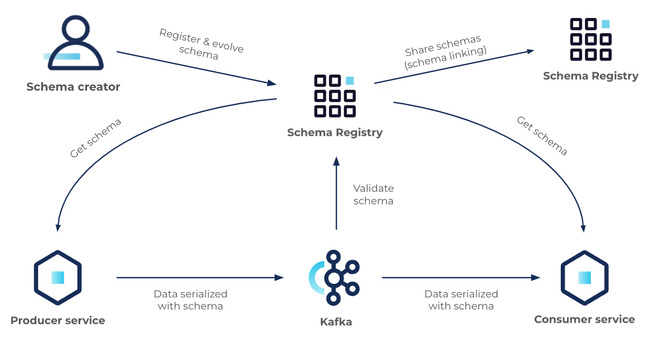
\includegraphics[width=0.9\textwidth]{../Images/SpecificaTecnica/schemaRegistry.jpg}
    \caption{Schema Registry overview - Confluent documentation}
    \label{fig:schemaReg}
\end{figure}

Schema Registry permette la convalida del formato dei messaggi per garantire l'integrità e l'affidabilità dei dati in \textit{Apache Kafka}\textsubscript{\textit{G}}.
\begin{enumerate}
    \item \textbf{Convalida dei messaggi:} Schema Registry convalida i messaggi in base allo schema registrato per il topic. I messaggi non validi vengono scartati;
    \item \textbf{Maggiore affidabilità:} La convalida dei messaggi aiuta a prevenire errori e a garantire che i dati siano conformi allo schema definito. Questo riduce il rischio di corruzione dei dati e di errori di elaborazione nei sistemi a valle;
    \item \textbf{Interoperabilità:} Schema Registry facilita la comunicazione tra diversi sistemi che producono e consumano messaggi \textit{Kafka}\textsubscript{\textit{G}}. Definendo un formato comune per i messaggi, i sistemi possono interoperare senza problemi, anche se sono sviluppati in linguaggi di programmazione diversi o utilizzano \textit{librerie}\textsubscript{\textit{G}} client differenti;
    \item \textbf{Evolutività:} Schema Registry permette di evolvere gli schemi dei messaggi nel tempo in modo compatibile. Ciò significa che è possibile aggiungere nuovi campi o modificare la struttura dei messaggi senza interrompere i sistemi esistenti;
    \item \textbf{Migliore debug:} La convalida dei messaggi fornisce informazioni utili in caso di errori, facilitando l'identificazione del problema e la sua risoluzione;
    \item \textbf{Sicurezza:} La convalida dei messaggi può essere utilizzata per proteggere il \textit{sistema}\textsubscript{\textit{G}} da messaggi malformati o dannosi.
\end{enumerate}

Convalida del formato dei messaggi con Schema Registry:
\begin{itemize}
    \item \textbf{Definizione dello schema:} Vengono definiti e registrati gli schemi per i messaggi \textit{Kafka}\textsubscript{\textit{G}} utilizzando il formato JSON;
    \item \textbf{Produzione dei messaggi:} I producer \textit{Kafka}\textsubscript{\textit{G}} inviano messaggi conformi allo schema definito per il topic di destinazione;
    \item \textbf{Convalida dei messaggi:} Schema Registry convalida i messaggi in base allo schema registrato per il topic, i messaggi non validi vengono scartati;
    \item \textbf{Consumo dei messaggi:} I consumer \textit{Kafka}\textsubscript{\textit{G}} ricevono solo messaggi convalidati.
\end{itemize}

\subsubsection{Schema dei messaggi}\label{sec:schema_registry_sez_schema}
I messaggi nei topic dedicati allo streaming delle misurazioni dei sensori devono essere nel seguente formato per superare la convalida definita da contratto nello Schema Registry.

\paragraph{Misurazioni dei senori}
\begin{lstlisting}[style=code]
    {
        "type": "record",
        "name": "Misurazione",
        "fields": [
          {
            "name": "timestamp",
            "type": "string"
          },
          {
            "name": "value",
            "type": "float"
          },
          {
            "name": "type",
            "type": "string"
          },
          {
            "name": "latitude",
            "type": "float"
          },
          {
            "name": "longitude",
            "type": "float"
          },
          {
            "name": "ID_sensore",
            "type": "string"
          },
          {
            "name": "cella",
            "type": "string"
          }
        ]
      }
\end{lstlisting}

\paragraph{Misurazioni del punteggio di salute}
I messaggi nel topic dedicato allo streaming delle misurazioni dei punteggi di salute devono essere nel seguente formato per superare la convalida definita da contratto nello Schema Registry.
\begin{lstlisting}[style=code]
    {
        "type": "record",
        "name": "MisurazioneSalute",
        "fields": [
          {
            "name": "timestamp",
            "type": "string"
          },
          {
            "name": "value",
            "type": "float"
          },
          {
            "name": "type",
            "type": "string"
          },
          {
            "name": "cella",
            "type": "string"
          }
        ]
      }
\end{lstlisting}

\paragraph{Implementazione Schema Registry}

Per registrare uno schema nel registro degli schemi di \textit{Kafka}\textsubscript{\textit{G}} viene utilizzato il comando \textit{curl} insieme alla \textit{Rest} \textit{API}\textsubscript{\textit{G}} fornita dallo schema registry.

Il comando \textit{curl} viene utilizzato tramite un'immagine \textit{Docker}\textsubscript{\textit{G}} dedicata.